\hypertarget{the-kalman-filter}{%
\section{The Kalman Filter}\label{the-kalman-filter}}

In this section we develop the multivariate version of the Kalman
Filter. The steps are basically the same as the scalar version described
in the last section, but the derivation is more involved.

\hypertarget{the-multivariate-version}{%
\subsection{The Multivariate Version}\label{the-multivariate-version}}

The \texttt{Kalman\ Filter} has two stages. A predictive step based on
the system dynamics and an update based on observations or measurements.

The full Kalman Filter has the following objects to track:

\begin{itemize}
\tightlist
\item
  \emph{Prediction}: \(\hat{x}_{k|k-1}\), \(P_{k|k-1}\)
\item
  \emph{Update}: \(\hat{x}_{k|k}\), \(P_{k|k}\)
\item
  \(P_{k|k} =  \textrm{cov}(x_k -  \hat{x}_{k|k})\)
\item
  \(P_{k|k-1} = \textrm{cov}(x_k - \hat{x}_{k|k-1})\)
\item
  \(S_{k} = \textrm{cov}(z_k - H\hat{x}_{k|k-1})\)
\end{itemize}

The prediction step uses the system dynamics, the linear dynamical
model, to predict where the system should be. This prediction is for
both the state estimate \(\hat{x}\) and the covariance of \(\hat{x}\).
This stage is also known as the \emph{a priori} since it occurs before
the observation.

The update step takes the observation at that step and compares it to
the prediction. The difference between the two is known as the
innovation. It is what is new compared to the system dynamics. Using a
weighted least squares approach, the two are merged. This is done by
determining how reliable the new information is based on the innovation
covariance. The weight term is known as the Kalman gain. The weighted
innovation is added to the prediction of the state estimate to obtain
the Kalman estimate. As before, this stage is also known as the \emph{a
posteriori} because it occurs after the observation. Repeated steps or
iterations of the Kalman filter allow the filter to track sequential
stages of a process. These sequential steps make this a recursive linear
gaussian state estimator.

Formally we have a dynamical process

\[x_{k+1} = F_k x_k + Gu_k + v_k\]

where \(F_k\) is the state transition matrix, \(Gu_k\) is the input
control and and observation

\[z_k = Hx_k + w_k\]

where \(H\) is the observation matrix. The random variables \(v_k\),
\(w_k\) are drawn from Gaussian distributions with covariance models
given by

\[V = E[v_kv_k^T], \quad\quad W = E[w_kw_k^T].\]

The error covariance of the estimate is

\[P_k = E[e_ke_k^T] = E[(x_k - \hat{x}_k)(x_k - \hat{x}_k)^T] .\]

The state estimate will be denoted \(\hat{x}_k\) and the process update
to the state is denoted \(\tilde{x}_k\)

Before we go into the details on the filter design, a couple of comments
about the matrices given in the dynamical process.

\begin{quote}
The matrix \(F\) is given by the model of the physical process. It is a
square matrix with dimension \(n \times n\) where \(n\) is the number of
state variables (the length of \(x\)). When you are given a continuous
dynamical system, make sure you first discretize the problem. Only then
can you extract the correct matrix \(F\).

The matrix \(G\) is more of a placeholder for now. We assume that we
have some type of control input \(Gu_k\) but for our discussion you
don't need to write this in any special form as long as you add the
control values into the process update. Meaning you don't need to figure
out matrix \(G\) to do the process update step.

The matrix \(H\) is the observation matrix. This acts to relate the
observed variables to the state variables. For example, say that you
have a state vector of \((x_1, x_2, x_3)\) and can observe all three as
\(z = (z_{x_1}, z_{x_2}, z_{x_3})\). Then

\[\begin{aligned}
H = \begin{bmatrix} 1 & 0 & 0 \\ 0 & 1 & 0\\ 0 & 0 &1 \end{bmatrix}.
\end{aligned}\]

However, if we observe \(x_1\) and \(x_3\) as \(z = (z_{x_1}, z_{x_3})\)
then

\[\begin{aligned}
H = \begin{bmatrix} 1 & 0 & 0 \\ 0 & 0 &1 \end{bmatrix}
\end{aligned}\]

or if we only observe \(x_2\) as \(z = (z_{x_2})\) then

\[H = \begin{bmatrix} 0 & 1 & 0  \end{bmatrix}\]

Note what the matrix \(H\) does in the following product \(H A H^T\) for
the observation \(z = (z_{x_1}, z_{x_3})\):

\[\begin{aligned}
H A H^T = \begin{bmatrix} 1 & 0 & 0 \\ 0 & 0 &1 \end{bmatrix}
\begin{bmatrix} a & b & c \\ d & e & f\\ g & h &i \end{bmatrix}
\begin{bmatrix} 1 & 0 \\ 0 & 0  \\ 0 & 1 \end{bmatrix}
=
\begin{bmatrix} 1 & 0 & 0 \\ 0 & 0 &1 \end{bmatrix}
\begin{bmatrix} a & c \\ d  & f\\ g &i \end{bmatrix}
=
\begin{bmatrix} a & c \\ g &i \end{bmatrix}
\end{aligned}\]
\end{quote}

Moving on to the derivation, we assume that we can write our estimate as
a combination of the process update and the observation

\[\hat{x}_k = \tilde{x}_k + K_k (z_k - H\tilde{x}_k)\]

The optimal choice of the Kalman gain parameter is to select \(K_k\) to
minimize the mean square error \(E[ \| x_k - \hat{x}_{k|k} \|^2 ]\). You
will notice that

\[E[ \| x_k - \hat{x}_{k|k} \| ] = E \left[ \sum_i (x^i_{k}- \hat{x}^i_{k|k})^2\right]
 = Tr(P_{k|k})\]

where \(Tr(P_{k|k})\) is the trace of \(P_{k|k}\). So, we need an
expression for \(P_{k|k}\) in terms of the Kalman gain.

We can plug in the observation, \texttt{kalmanderivation1} into
\texttt{kalmanderivation4}

\[\hat{x}_k = \tilde{x}_k + K_k (Hx_k + w_k - H\tilde{x}_k)\]

This form of the estimate can be substituted into the error covariance

\[P_{k|k} = E[e_ke_k^T] = E[[(I - K_kH)(x_k-\tilde{x}_k)-K_kw_k][(I - K_kH)(x_k-\tilde{x}_k)-K_kw_k]^T] .\]

Since observation or measurement noise is not correlated to process
noise we can rewite

\[P_{k|k} = (I - K_kH) E[(x_k-\tilde{x}_k)(x_k-\tilde{x}_k)^T](I - K_kH)^T -  K_kE[w_kw_k^T] K_k^T.\]

Since \(P_{k|k-1} = E[(x_k-\tilde{x}_k)(x_k-\tilde{x}_k)^T]\) we obtain

\[P_{k|k} = (I - K_kH) P_{k|k-1} (I - K_kH)^T -  K_k W K_k^T .\]

Expanding the expression and using \(S_k = H P_{k|k-1} H^T + W_k\) we
have

\[P_{k|k}  = P_{k|k-1}  - K_kH P_{k|k-1} - P_{k|k-1} H^T K_K^T + K_k S_k K_k^T\]

As stated above, we want to minimize \(Tr(P_{k|k})\) with respect to
\(K_k\):

\[\frac{\partial Tr(P_{k|k})}{\partial K_k} = -2(H P_{k|k-1})^T + 2K_k S_k = 0,\]

solving for the Kalman gain gives

\[K_k = P_{k|k-1}H^T S^{-1}_k .\]

We can collect the results into the following algorithm:

\textbf{Kalman Filter}

\textbf{Predict:} Prediction or a priori stage

\begin{itemize}
\tightlist
\item
  Predicted state:
  \(\hat{x}_{k|k-1} = F_{k}\hat{x}_{k-1|k-1} + G_{k} u_{k}\)
\item
  Predicted estimate covariance:
  \(P_{k|k-1} = F_{k} P_{k-1|k-1} F_{k}^{T} + V_{k}\)
\end{itemize}

\textbf{Update:} Update or a posteriori stage

\begin{itemize}
\tightlist
\item
  \texttt{Innovation\ residual} or \texttt{measurement\ residual}:
  \(y_k = z_k - H_k\hat{x}_{k|k-1}\)
\item
  Innovation (or residual) covariance:
  \(S_k = H_k P_{k|k-1} H_k^\text{T} + W_k\)
\item
  \texttt{Optimal\ Kalman\ gain}:
  \(K_k = P_{k|k-1}H_k^\text{T}S_k^{-1}\)
\item
  Updated state estimate \(\hat{x}_{k|k} =\hat{x}_{k|k-1} + K_k y_k\)
\item
  Updated estimate covariance: \(P_{k|k} = (I - K_k H_k) P_{k|k-1}\)
\end{itemize}

The control input is the current control input and depends on how you
index it as to being \(u_k\) or \(u_{k-1}\). You can think of this
control being injected between \(k\) and \(k-1\). So it is not critical
how you index the term and will be clear from the process equations.

If the model is accurate, and the values for \(\hat{x}_{0|0}\)

and \(P_{0|0}\) accurately reflect the distribution of the initial state
values, then the following invariants are preserved: (all estimates have
mean error zero)

\begin{itemize}
\tightlist
\item
  \(\textrm{E}[x_k - \hat{x}_{k|k}] =\textrm{E}[x_k - \hat{x}_{k|k-1}] = 0\)
\item
  \(\textrm{E}[z_k] = 0\)
\end{itemize}

where \(E[\xi]\) is the expected value of \(\xi\).

Assume that you have the following Gaussian process and observation:

\[\begin{aligned}
\begin{array}{l}
x_k = Fx_{k-1} + Gu_k + v_k\\
z_k = Hx_k + w_k
\end{array}
\end{aligned}\]

then

\begin{quote}
\textbf{Input} \(x_0\), \(P_0\)\\
\textbf{Output} Estimates of \(x_k\), \(P_k\)\\
\(k=0\)\\
\textbf{while} (not terminated) \textbf{do}\\
\hspace*{0.333em}\hspace*{0.333em}\hspace*{0.333em}\(k=k+1\)\\
\hspace*{0.333em}\hspace*{0.333em}\hspace*{0.333em}\(x_k = F_{k}x_{k-1} + G_{k} u_{k}\)\\
\hspace*{0.333em}\hspace*{0.333em}\hspace*{0.333em}\(P_{k} = F_{k} P_{k-1} F_{k}^{T} + V_{k}\)\\
\hspace*{0.333em}\hspace*{0.333em}\hspace*{0.333em}\(y_k = z_k - H_kx_{k}\)\\
\hspace*{0.333em}\hspace*{0.333em}\hspace*{0.333em}\(S_k = H_k P_{k} H_k^\text{T} + W_k\)\\
\hspace*{0.333em}\hspace*{0.333em}\hspace*{0.333em}\(K_k = P_{k}H_k^\text{T}S_k^{-1}\)\\
\hspace*{0.333em}\hspace*{0.333em}\hspace*{0.333em}\(x_k =   x_{k} + K_k y_k\)\\
\hspace*{0.333em}\hspace*{0.333em}\hspace*{0.333em}\(P_{k} = (I - K_k H_k) P_{k}\)\\
\textbf{end while}
\end{quote}

\begin{figure}
\centering
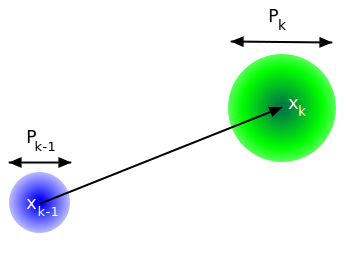
\includegraphics[width=0.5\textwidth,height=\textheight]{AdvFilteringFigures/pointmapcloud.*}
\caption{Single Step of Kalman process.}
\end{figure}

The Kalman code generally looks like

\begin{Shaded}
\begin{Highlighting}[]
\KeywordTok{for}\NormalTok{ k }\OperatorTok{=} \FloatTok{2}\OperatorTok{:}\NormalTok{N}
\NormalTok{  x\_process\_update }\OperatorTok{=}\NormalTok{ F }\OperatorTok{*}\NormalTok{ x\_estimate[k}\OperatorTok{{-}}\FloatTok{1}\NormalTok{] }\OperatorTok{+}\NormalTok{ G[k]}
\NormalTok{  P\_variance\_update }\OperatorTok{=}\NormalTok{ F }\OperatorTok{*}\NormalTok{ (P\_variance[k}\OperatorTok{{-}}\FloatTok{1}\NormalTok{] }\OperatorTok{*}\NormalTok{ FT) }\OperatorTok{+}\NormalTok{ V}
\NormalTok{  innovation }\OperatorTok{=}\NormalTok{ z\_observation[k] }\OperatorTok{{-}}\NormalTok{ H }\OperatorTok{*}\NormalTok{ x\_process\_update}
\NormalTok{  Innovation\_covariance }\OperatorTok{=}\NormalTok{ H }\OperatorTok{*}\NormalTok{ (P\_variance\_update }\OperatorTok{*}\NormalTok{ HT) }\OperatorTok{+}\NormalTok{ W}
\NormalTok{  Kal\_gain }\OperatorTok{=}\NormalTok{ P\_variance\_update }\OperatorTok{*}\NormalTok{ (HT }\OperatorTok{*}\NormalTok{ inv(Innovation\_covariance) )}
\NormalTok{  x\_estimate[k] }\OperatorTok{=}\NormalTok{ x\_process\_update }\OperatorTok{+}\NormalTok{ Kal\_gain }\OperatorTok{*}\NormalTok{ y}
\NormalTok{  P\_variance[k] }\OperatorTok{=}\NormalTok{ P\_variance\_update }\OperatorTok{{-}}\NormalTok{ Kal\_gain }\OperatorTok{*}\NormalTok{ (H }\OperatorTok{*}\NormalTok{ P\_variance\_update )}
\KeywordTok{end}
\end{Highlighting}
\end{Shaded}

\hypertarget{simple-example-of-a-single-step}{%
\subsection{Simple Example of a Single
Step}\label{simple-example-of-a-single-step}}

Let

\[\begin{aligned}
x = \begin{bmatrix}a \\ b\end{bmatrix}, \quad F = \begin{bmatrix} 0.9 &-.01 \\0.02 &0.75\end{bmatrix},
\quad G = \begin{bmatrix} 0.1\\ 0.05\end{bmatrix}, \quad H = \begin{bmatrix} 1& 0 \end{bmatrix},
\end{aligned}\]

\[\begin{aligned}
V = \begin{bmatrix} 0.005265&0\\0& 0.005265\end{bmatrix}, \quad W = 0.7225,\quad z_1 = 0.01
\end{aligned}\]

\[\begin{aligned}
\quad u_k = \sin (7*k/100), \quad x_0 = \begin{bmatrix} 0\\0\end{bmatrix},
\quad P_0 = \begin{bmatrix}0 & 0\\ 0&0\end{bmatrix}.
\end{aligned}\]

Apply the Kalman Filter process and compute \(\hat{x}_{1|1}\) and
\(P_{1|1}\).

Process update:

\[\begin{aligned}
\hat{x}_{1|0} = \begin{bmatrix} 0.9 &-.01 \\0.02 &0.75\end{bmatrix}\hat{x}_{0|0}
+ \begin{bmatrix} 0.1\\ 0.05\end{bmatrix} u_k
=  \begin{bmatrix} 0.9 &-.01 \\0.02 &0.75\end{bmatrix}\begin{bmatrix} 0\\0\end{bmatrix}
+ \begin{bmatrix} 0.1\\ 0.05\end{bmatrix}\sin (7/100)
\end{aligned}\]

\[\begin{aligned}
\approx \begin{bmatrix} 0.0069942847\\  0.0034971424\end{bmatrix}
\end{aligned}\]

Process covariance update:

\[P_{1|0} = F P_{0|0} F^{T} + V =\]

\[\begin{aligned}
P_{1|0} = \begin{bmatrix} 0.9 &-.01 \\0.02 &0.75\end{bmatrix}\begin{bmatrix}0 & 0\\ 0&0\end{bmatrix} \begin{bmatrix} 0.9 &0.02 \\ -.01&0.75\end{bmatrix} +\begin{bmatrix} 0.005265&0\\0& 0.005265\end{bmatrix}
\end{aligned}\]

\[\begin{aligned}
= \begin{bmatrix} 0.005265&0\\0& 0.005265\end{bmatrix}.
\end{aligned}\]

Innovation and innovation covariance:

\[\begin{aligned}
y_1 = 0.01 - \begin{bmatrix} 1& 0 \end{bmatrix}\hat{x}_{1|0} = 0.01 - \begin{bmatrix} 1& 0 \end{bmatrix}\begin{bmatrix} 0.0069942847\\  0.0034971424\end{bmatrix}
\end{aligned}\]

\[= 0.0030057153\]

\[\begin{aligned}
S_1 = HP_{1|0} H^\text{T} + W = \begin{bmatrix} 1 & 0\end{bmatrix} \begin{bmatrix} 0.005265&0\\0& 0.005265\end{bmatrix}\begin{bmatrix} 1\\0\end{bmatrix} + 0.7225
\end{aligned}\]

\[=0.728125\]

Kalman Gain

\[\begin{aligned}
K_1 = P_{1|0}H_1^\text{T}S_1^{-1} = \begin{bmatrix} 0.005265&0\\0& 0.005265\end{bmatrix}
\begin{bmatrix} 1\\0\end{bmatrix}/0.728125
\end{aligned}\]

\[\begin{aligned}
= \begin{bmatrix} 0.00772532 \\ 0.0 \end{bmatrix}
\end{aligned}\]

Updated state variables

\[\begin{aligned}
\hat{x}_{1|1} =
  \hat{x}_{1|0} + K_1 y_1 = \begin{bmatrix} 0.0069942847\\  0.0034971424\end{bmatrix} + \begin{bmatrix} 0.00772532 \\ 0.0 \end{bmatrix} (0.00300572)
\end{aligned}\]

\[\begin{aligned}
= \begin{bmatrix} 0.007017504813\\  0.0034971424\end{bmatrix}
\end{aligned}\]

State variable covariance:

\[\begin{aligned}
P_{1|1} =
  (I - K_1 H_1) P_{1|0} =  \begin{bmatrix} 0.99227468 & 0.0 \\ 0.0 & 1.0 \end{bmatrix} P_{1|0}
\end{aligned}\]

\[\begin{aligned}
= \begin{bmatrix} 0.005224326  &  0.0 \\
0.0  &  0.005265 \end{bmatrix}
\end{aligned}\]

It is useful to visualize the effects of a single Kalman step. The
images are provided in \texttt{fig:kalmanclouds1} -
~\texttt{fig:kalmanclouds3} and the numbers used are not the same as the
example above\footnote{The numbers were selected to help visualize the
  process.}. The system we use is Let

\[\begin{aligned}
x_0 = \begin{bmatrix} 1\\1\end{bmatrix}, \quad P_0 = \begin{bmatrix}0.01& 0\\ 0&0.001\end{bmatrix}, \quad F = \begin{bmatrix} 0.85 &-.1 \\0.02 &0.75\end{bmatrix},
\end{aligned}\]

\[\begin{aligned}
G = \begin{bmatrix} 0.025\\ 0.05\end{bmatrix}, \quad H = I,
 V = \begin{bmatrix} 0.0075^2&0\\0& 0.0075^2\end{bmatrix},
\end{aligned}\]

\[\begin{aligned}
W = \begin{bmatrix} 0.035^2&0\\0& 0.035^2\end{bmatrix}, \quad  a = \begin{bmatrix} 0.01\\ 0.02\end{bmatrix} ,\quad z = \hat{x}  +a+ w_k.
\end{aligned}\]

\begin{figure}
\centering
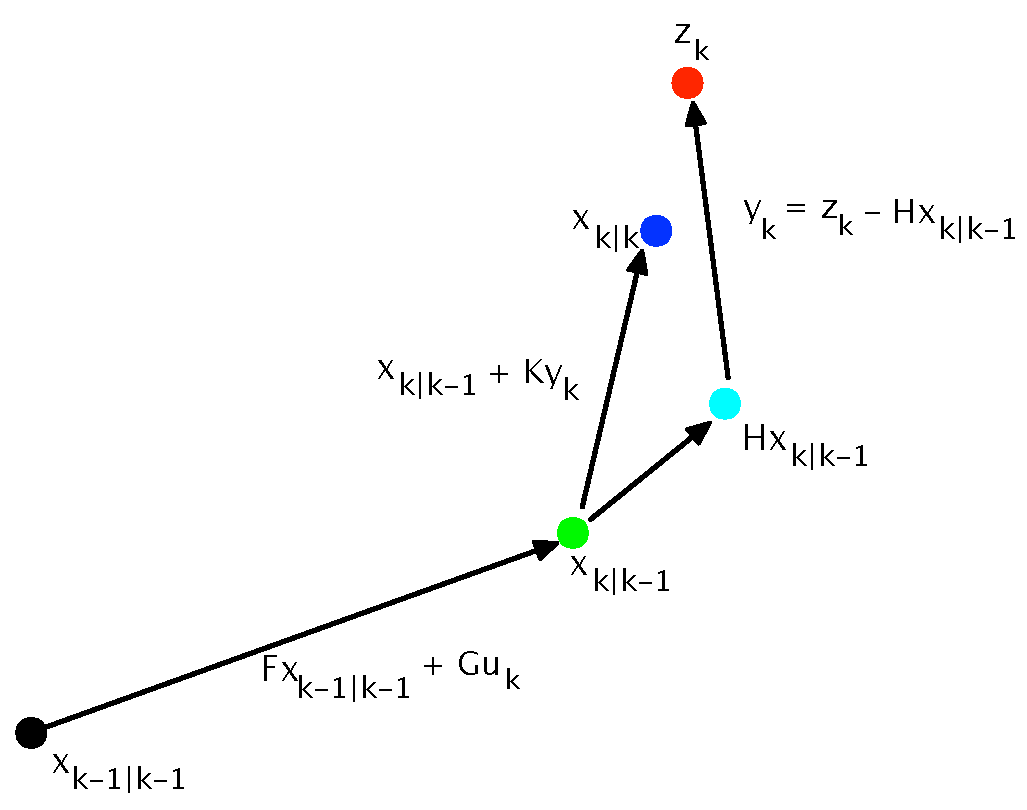
\includegraphics[width=0.65\textwidth,height=\textheight]{AdvFilteringFigures/kalmanupdatedia.*}
\caption{Parts of the single Kalman step - estimate.}
\end{figure}

\begin{figure}
\centering
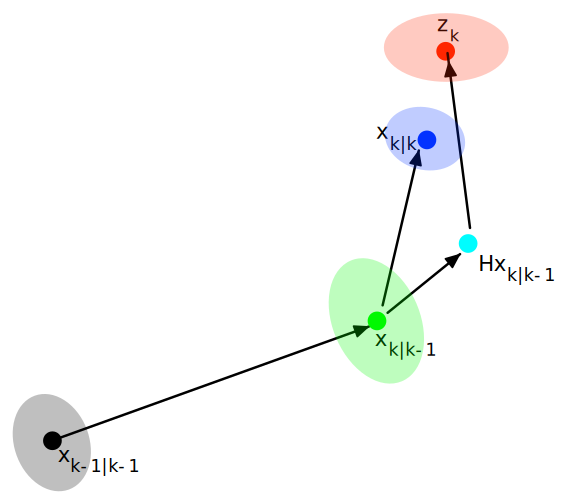
\includegraphics[width=0.65\textwidth,height=\textheight]{AdvFilteringFigures/kalmanupdatedia2.*}
\caption{Parts of the single Kalman step - covariances.}
\end{figure}

Starting with a single point, we move this forward using the process
update. From the same starting point we run each forward with the
process update, \(\hat{x}_{k|k-1}\) many times to generate a
distribution. The resulting points are different since the process
update has noise. \texttt{fig:kalmanclouds1} shows the point cloud (in
blue). This process does not have a great deal of noise so the cloud is
tightly clustered. \texttt{fig:kalmanclouds2} shows the observation
\(z_k\). \texttt{fig:kalmanclouds3} shows the observation update, the
fusion of the observation with the state update.

\begin{Shaded}
\begin{Highlighting}[]
\KeywordTok{using}\NormalTok{ Plots}\OperatorTok{,} \BuiltInTok{Random}\OperatorTok{,}\NormalTok{ Distributions}
\NormalTok{M }\OperatorTok{=} \FloatTok{250}
\NormalTok{F }\OperatorTok{=}\NormalTok{ [}\FloatTok{0.85} \OperatorTok{{-}}\FloatTok{0.1} \OperatorTok{;} \FloatTok{0.02} \FloatTok{0.75}\NormalTok{]}
\NormalTok{FT }\OperatorTok{=}\NormalTok{ transpose(F)}
\NormalTok{a }\OperatorTok{=}\NormalTok{ [}\FloatTok{0.01} \OperatorTok{;} \FloatTok{0.02}\NormalTok{]}
\NormalTok{G }\OperatorTok{=}\NormalTok{ [}\FloatTok{0.025}\OperatorTok{,}\FloatTok{0.05}\NormalTok{]}
\NormalTok{x\_initial }\OperatorTok{=}\NormalTok{ [}\FloatTok{1} \OperatorTok{;} \FloatTok{1}\NormalTok{]}
\NormalTok{P\_initial }\OperatorTok{=}\NormalTok{ [}\FloatTok{0.01} \FloatTok{0.0} \OperatorTok{;} \FloatTok{0.0} \FloatTok{0.001}\NormalTok{]}
\NormalTok{mu1}\OperatorTok{,}\NormalTok{ mu2 }\OperatorTok{=} \FloatTok{0.0}\OperatorTok{,} \FloatTok{0.0}
\NormalTok{sigma1}\OperatorTok{,}\NormalTok{ sigma2 }\OperatorTok{=} \FloatTok{0.0075}\OperatorTok{,} \FloatTok{0.035}
\NormalTok{var1 }\OperatorTok{=}\NormalTok{ sigma1}\OperatorTok{*}\NormalTok{sigma1}
\NormalTok{var2 }\OperatorTok{=}\NormalTok{ sigma2}\OperatorTok{*}\NormalTok{sigma2}
\NormalTok{r1 }\OperatorTok{=}\NormalTok{ Normal(mu1}\OperatorTok{,}\NormalTok{sigma1)}
\NormalTok{r2 }\OperatorTok{=}\NormalTok{ Normal(mu2}\OperatorTok{,}\NormalTok{sigma2)}
\NormalTok{V }\OperatorTok{=}\NormalTok{ [var1 }\FloatTok{0.0} \OperatorTok{;} \FloatTok{0.0}\NormalTok{ var1]}
\NormalTok{W }\OperatorTok{=}\NormalTok{ [var2 }\FloatTok{0.0} \OperatorTok{;} \FloatTok{0.0}\NormalTok{ var2]}
\NormalTok{x\_apriori }\OperatorTok{=} \DataTypeTok{Vector}\NormalTok{\{}\DataTypeTok{Float64}\NormalTok{\}()}
\NormalTok{y\_apriori }\OperatorTok{=} \DataTypeTok{Vector}\NormalTok{\{}\DataTypeTok{Float64}\NormalTok{\}()}
\NormalTok{obsx }\OperatorTok{=} \DataTypeTok{Vector}\NormalTok{\{}\DataTypeTok{Float64}\NormalTok{\}()}
\NormalTok{obsy}\OperatorTok{=} \DataTypeTok{Vector}\NormalTok{\{}\DataTypeTok{Float64}\NormalTok{\}()}
\NormalTok{x\_post }\OperatorTok{=} \DataTypeTok{Vector}\NormalTok{\{}\DataTypeTok{Float64}\NormalTok{\}()}
\NormalTok{y\_post }\OperatorTok{=} \DataTypeTok{Vector}\NormalTok{\{}\DataTypeTok{Float64}\NormalTok{\}()}


\KeywordTok{for}\NormalTok{ i }\OperatorTok{=} \FloatTok{1}\OperatorTok{:}\NormalTok{M}
\NormalTok{  x\_process\_update }\OperatorTok{=}\NormalTok{ F}\OperatorTok{*}\NormalTok{x\_initial  }\OperatorTok{+}\NormalTok{ G }\OperatorTok{+}\NormalTok{ rand(r1}\OperatorTok{,} \FloatTok{2}\NormalTok{)}
  \ConstantTok{append}\OperatorTok{!}\NormalTok{(x\_apriori}\OperatorTok{,}\NormalTok{x\_process\_update[}\FloatTok{1}\NormalTok{])}
  \ConstantTok{append}\OperatorTok{!}\NormalTok{(y\_apriori}\OperatorTok{,}\NormalTok{x\_process\_update[}\FloatTok{2}\NormalTok{])}
\NormalTok{  P\_variance\_update }\OperatorTok{=}\NormalTok{ F}\OperatorTok{*}\NormalTok{P\_initial}\OperatorTok{*}\NormalTok{FT }\OperatorTok{+}\NormalTok{ V}
\NormalTok{  z\_test\_data }\OperatorTok{=}\NormalTok{ F}\OperatorTok{*}\NormalTok{x\_initial  }\OperatorTok{+}\NormalTok{ G  }\OperatorTok{+}\NormalTok{ a }\OperatorTok{+}\NormalTok{ rand(r2}\OperatorTok{,}\FloatTok{2}\NormalTok{)}
  \ConstantTok{append}\OperatorTok{!}\NormalTok{(obsx}\OperatorTok{,}\NormalTok{z\_test\_data[}\FloatTok{1}\NormalTok{])}
  \ConstantTok{append}\OperatorTok{!}\NormalTok{(obsy}\OperatorTok{,}\NormalTok{z\_test\_data[}\FloatTok{2}\NormalTok{])}

\NormalTok{  innovation }\OperatorTok{=}\NormalTok{ z\_test\_data }\OperatorTok{{-}}\NormalTok{ x\_process\_update}
\NormalTok{  Innovation\_variance }\OperatorTok{=}\NormalTok{ P\_variance\_update }\OperatorTok{+}\NormalTok{ W}

\NormalTok{  kal\_gain }\OperatorTok{=}\NormalTok{ P\_variance\_update}\OperatorTok{*}\NormalTok{inv(Innovation\_variance)}
\NormalTok{  x\_filter }\OperatorTok{=}\NormalTok{ x\_process\_update }\OperatorTok{+}\NormalTok{ kal\_gain}\OperatorTok{*}\NormalTok{innovation}

  \ConstantTok{append}\OperatorTok{!}\NormalTok{(x\_post}\OperatorTok{,}\NormalTok{x\_filter[}\FloatTok{1}\NormalTok{])}
  \ConstantTok{append}\OperatorTok{!}\NormalTok{(y\_post}\OperatorTok{,}\NormalTok{x\_filter[}\FloatTok{2}\NormalTok{])}

\KeywordTok{end}

\NormalTok{scatter(x\_apriori}\OperatorTok{,}\NormalTok{y\_apriori}\OperatorTok{,}\NormalTok{ xlim}\OperatorTok{=}\NormalTok{(}\FloatTok{0.7}\OperatorTok{,}\FloatTok{0.95}\NormalTok{)}\OperatorTok{,}\NormalTok{ ylim}\OperatorTok{=}\NormalTok{(}\FloatTok{0.7}\OperatorTok{,} \FloatTok{0.95}\NormalTok{)}\OperatorTok{,}\NormalTok{ aspect\_ratio }\OperatorTok{=} \FloatTok{1.0}\NormalTok{)}
\NormalTok{scatter}\OperatorTok{!}\NormalTok{(obsx}\OperatorTok{,}\NormalTok{obsy}\OperatorTok{,}\NormalTok{ xlim}\OperatorTok{=}\NormalTok{(}\FloatTok{0.7}\OperatorTok{,}\FloatTok{0.95}\NormalTok{)}\OperatorTok{,}\NormalTok{ ylim}\OperatorTok{=}\NormalTok{(}\FloatTok{0.7}\OperatorTok{,} \FloatTok{0.95}\NormalTok{)}\OperatorTok{,}\NormalTok{ aspect\_ratio }\OperatorTok{=} \FloatTok{1.0}\NormalTok{)}
\NormalTok{scatter}\OperatorTok{!}\NormalTok{(x\_post}\OperatorTok{,}\NormalTok{y\_post}\OperatorTok{,}\NormalTok{ xlim}\OperatorTok{=}\NormalTok{(}\FloatTok{0.7}\OperatorTok{,}\FloatTok{0.95}\NormalTok{)}\OperatorTok{,}\NormalTok{ ylim}\OperatorTok{=}\NormalTok{(}\FloatTok{0.7}\OperatorTok{,} \FloatTok{0.95}\NormalTok{)}\OperatorTok{,}\NormalTok{ aspect\_ratio }\OperatorTok{=} \FloatTok{1.0}\NormalTok{)}
\end{Highlighting}
\end{Shaded}

You will notice that it is not circular. The covariance matrix really
trusted the \(y\) process estimate and so weighted the process more than
the observation. In the \(x\) estimate, much more of the observation was
used. So the resulting point cloud has lower variation in \(y\) than
\(x\). \texttt{fig:kalmanclouds4} graphs the error ellipses for the
previous point clouds. It is easier to see the changes from this than
looking at the raw data.

\begin{quote}
Point distribution after process update.

Observed point distribution.

Final distribution after update step.

The standard deviation based ellipses.
\end{quote}

\hypertarget{generation-of-testing-data}{%
\subsection{Generation of Testing
Data}\label{generation-of-testing-data}}

\begin{figure}
\centering
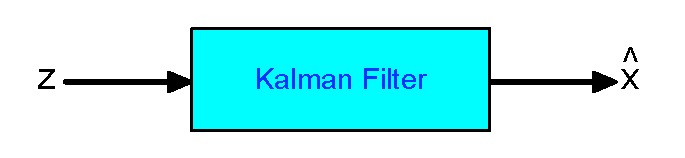
\includegraphics[width=0.5\textwidth,height=\textheight]{AdvFilteringFigures/kalmanblock.*}
\caption{Kalman Code as a black box.}
\end{figure}

The development of filtering software needs to have datasets to test the
software. The early stages of software development are about removing
simple errors such as syntax errors. In the absence of a real robot
producing actual data, how do we develop and test our code? This can be
done using pure simulation. We can simulate the motion of a robot. In
practice we just compute the location and orientation of the robot based
on the motion equations or kinematics derived in the Motion chapter. For
example, for the differential drive robot, we can send control signals
(the wheel speeds) and compute the location of the robot. Each step of
the simulation produces a small motion and a small amount of error. That
error will accumulate which is consistent with what we see in actual
systems. Assume that the robot moves along according to the kinematic
model \(F\) and \(G\) plus the noise, we have

\[x_{k+1} = Fx_k + Gu_k + v_k\]

This produces the robot path as a vector of values \(\{ x \}\).

At each step along the computed path, we can make an observation
(\(z_k\)) which is noise added to the exact values \(x_k + v_k\) where
\(v_k\) is Gaussian noise. Since \(z_k\) is not added back into the
computation for \(x_{k+1}\), the observation noise, \(w_k\), does not
accumulate. The process is the following:

\[x_{k+1} = Fx_k + Gu_k + v_k\]

\[z_{k+1} = Hx_k + w_k\]

\begin{figure}
\centering
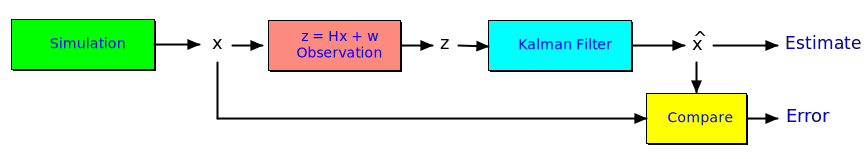
\includegraphics[width=0.95\textwidth,height=\textheight]{AdvFilteringFigures/KalmanSimulationBlock.*}
\caption{Simulation and testing.}
\end{figure}

The point is that the observations \(z\) can be computed after we
compute the \(x\) values or they can be computed together in the loop.
It does not matter in this case.

\hypertarget{kalman-code-examples}{%
\subsection{Kalman Code Examples}\label{kalman-code-examples}}

For this next example we modify the last example in a couple of ways. We
will observe both variables. This will have the effect of making the
innovation covariance \(S\) a matrix and we will need to compute a
matrix inverse. Next we will use a non-diagonal noise covariance for
\(V\) and \(W\).

We use these values to run a simulation which then produces the
observations we need to feed into the Kalman filter. The code block
below will generate a list of values which can be used as the
observations for a run of a Kalman filtering algorithm. Let

\[\begin{aligned}
x = \begin{bmatrix}a \\ b\end{bmatrix}, \quad
F = \begin{bmatrix} 0.85 &-.01 \\0.02 &0.65\end{bmatrix}, \quad
H = \begin{bmatrix} 1& 0 \\ 0 & 1 \end{bmatrix},
\end{aligned}\]

\[\begin{aligned}
V = \begin{bmatrix} 0.2 & 0.02 \\ 0.02 & 0.35 \end{bmatrix}, \quad
W = \begin{bmatrix}  0.4 & 0.0 \\ 0.0 & 0.4  \end{bmatrix} .
\end{aligned}\]

\[\begin{aligned}
\quad Gu_k = \begin{bmatrix}0.75\sin(0.5t_k) \\ 0.5\cos(0.5t_k) \end{bmatrix}, \quad
x_0 = \begin{bmatrix} 0\\0\end{bmatrix}, \quad
P_0 = \begin{bmatrix}0 & 0\\ 0&0\end{bmatrix}.
\end{aligned}\]

Assume that you want to simulate this on \(0 \leq t \leq 10\) with 200
subdivisions. The includes ...

\begin{Shaded}
\begin{Highlighting}[]
\KeywordTok{using} \BuiltInTok{Random}\OperatorTok{,}\NormalTok{ Distributions}
\KeywordTok{using}\NormalTok{ Plots}\OperatorTok{,}\NormalTok{ LinearAlgebra}
\end{Highlighting}
\end{Shaded}

The simulation variables ... (note \(t = 0.05*k\))

\begin{Shaded}
\begin{Highlighting}[]
\CommentTok{\#  Create fake dataset for experiment}
\NormalTok{N }\OperatorTok{=} \FloatTok{200}
\NormalTok{t }\OperatorTok{=}\NormalTok{ range(}\FloatTok{0}\OperatorTok{,} \FloatTok{10}\OperatorTok{,}\NormalTok{ length }\OperatorTok{=}\NormalTok{ N)  }\CommentTok{\# for control input}
\NormalTok{u1 }\OperatorTok{=} \FloatTok{0.75}\OperatorTok{*}\NormalTok{sin.(}\FloatTok{0.5}\OperatorTok{*}\NormalTok{t)}
\NormalTok{u2 }\OperatorTok{=} \FloatTok{0.5}\OperatorTok{*}\NormalTok{cos.(}\FloatTok{0.5}\OperatorTok{*}\NormalTok{t)}
\NormalTok{mu1 }\OperatorTok{=}\NormalTok{ [}\FloatTok{0.0}\OperatorTok{,} \FloatTok{0.0}\NormalTok{]}
\NormalTok{mu2 }\OperatorTok{=}\NormalTok{ [}\FloatTok{0.0}\OperatorTok{,} \FloatTok{0.0}\NormalTok{]}
\NormalTok{x\_sim }\OperatorTok{=}\NormalTok{ zeros(}\FloatTok{2}\OperatorTok{,}\NormalTok{ N)}
\NormalTok{z\_sim }\OperatorTok{=}\NormalTok{ zeros(}\FloatTok{2}\OperatorTok{,}\NormalTok{ N)}
\NormalTok{F }\OperatorTok{=} \DataTypeTok{Float64}\NormalTok{[}\FloatTok{0.85} \OperatorTok{{-}}\FloatTok{0.01}\OperatorTok{;} \FloatTok{0.02} \FloatTok{0.65}\NormalTok{]}
\NormalTok{FT }\OperatorTok{=}\NormalTok{ transpose(F)}
\NormalTok{G }\OperatorTok{=}\NormalTok{ transpose(}\DataTypeTok{Float64}\NormalTok{[u1 u2}\OperatorTok{;}\NormalTok{])}
\end{Highlighting}
\end{Shaded}

The filter variables

\begin{Shaded}
\begin{Highlighting}[]
\NormalTok{H }\OperatorTok{=} \DataTypeTok{Float64}\NormalTok{[}\FloatTok{1} \FloatTok{0}\OperatorTok{;} \FloatTok{0} \FloatTok{1}\NormalTok{]}
\NormalTok{HT }\OperatorTok{=}\NormalTok{ transpose(H)}
\NormalTok{V }\OperatorTok{=} \DataTypeTok{Float64}\NormalTok{[}\FloatTok{0.2} \FloatTok{0.02}\OperatorTok{;} \FloatTok{0.02} \FloatTok{0.35}\NormalTok{]}
\NormalTok{W }\OperatorTok{=} \DataTypeTok{Float64}\NormalTok{[}\FloatTok{0.4} \FloatTok{0.0}\OperatorTok{;} \FloatTok{0.0} \FloatTok{0.4}\NormalTok{]}
\NormalTok{P }\OperatorTok{=}\NormalTok{ zeros(}\FloatTok{2}\OperatorTok{,}\FloatTok{2}\NormalTok{)}
\NormalTok{x\_estimate }\OperatorTok{=}\NormalTok{ zeros(}\FloatTok{2}\OperatorTok{,}\NormalTok{N)}
\end{Highlighting}
\end{Shaded}

In practice you will simplify some of the expressions before coding them
up. For example, the matrix \(H\) is the identity matrix and you can
just remove it. It is left in so you can see the full process just like
it appears in the original algorithm. Also, if you cat/paste the code,
you have it.

The simulation ...

\begin{Shaded}
\begin{Highlighting}[]
\KeywordTok{for}\NormalTok{ k }\OperatorTok{=} \FloatTok{2}\OperatorTok{:}\NormalTok{N}
\NormalTok{  process\_noise }\OperatorTok{=}\NormalTok{ rand(MvNormal(mu1}\OperatorTok{,}\NormalTok{ V)}\OperatorTok{,} \FloatTok{1}\NormalTok{)}
\NormalTok{  observation\_noise }\OperatorTok{=}\NormalTok{ rand(MvNormal(mu2}\OperatorTok{,}\NormalTok{ W)}\OperatorTok{,} \FloatTok{1}\NormalTok{)}
\NormalTok{  x\_sim[}\OperatorTok{:,}\NormalTok{k] }\OperatorTok{=}\NormalTok{ (F }\OperatorTok{*}\NormalTok{ x\_sim[}\OperatorTok{:,}\NormalTok{ k}\OperatorTok{{-}}\FloatTok{1}\NormalTok{]) }\OperatorTok{+}\NormalTok{ G[}\OperatorTok{:,}\NormalTok{k] }\OperatorTok{+}\NormalTok{ process\_noise}
\NormalTok{  z\_sim[}\OperatorTok{:,}\NormalTok{k] }\OperatorTok{=}\NormalTok{ (H }\OperatorTok{*}\NormalTok{ x\_sim[}\OperatorTok{:,}\NormalTok{ k]) }\OperatorTok{+}\NormalTok{ observation\_noise}
 \KeywordTok{end}
 \CommentTok{\# done with fake data}
\end{Highlighting}
\end{Shaded}

The code block above provides the array z which is then piped into the
Kalman Filter

\begin{Shaded}
\begin{Highlighting}[]
\KeywordTok{for}\NormalTok{ k }\OperatorTok{=} \FloatTok{2}\OperatorTok{:}\NormalTok{N}
\NormalTok{  x\_process\_update }\OperatorTok{=}\NormalTok{ F }\OperatorTok{*}\NormalTok{ x\_estimate[}\OperatorTok{:,}\NormalTok{k}\OperatorTok{{-}}\FloatTok{1}\NormalTok{] }\OperatorTok{+}\NormalTok{ G[}\OperatorTok{:,}\NormalTok{k]}
\NormalTok{  P\_variance\_update }\OperatorTok{=}\NormalTok{ F }\OperatorTok{*}\NormalTok{ (P }\OperatorTok{*}\NormalTok{ FT) }\OperatorTok{+}\NormalTok{ V}
\NormalTok{  innovation }\OperatorTok{=}\NormalTok{ z\_sim[}\OperatorTok{:,}\NormalTok{k] }\OperatorTok{{-}}\NormalTok{ H }\OperatorTok{*}\NormalTok{ x\_process\_update}
\NormalTok{  Innovation\_covariance }\OperatorTok{=}\NormalTok{ H }\OperatorTok{*}\NormalTok{ (P\_variance\_update }\OperatorTok{*}\NormalTok{ HT) }\OperatorTok{+}\NormalTok{ W}
\NormalTok{  Kal\_gain }\OperatorTok{=}\NormalTok{ P\_variance\_update }\OperatorTok{*}\NormalTok{ (HT }\OperatorTok{*}\NormalTok{ inv(Innovation\_covariance))}
\NormalTok{  x\_estimate[}\OperatorTok{:,}\NormalTok{k] }\OperatorTok{=}\NormalTok{ x\_process\_update }\OperatorTok{+}\NormalTok{ Kal\_gain }\OperatorTok{*}\NormalTok{ innovation}
\NormalTok{  P }\OperatorTok{=}\NormalTok{ P\_variance\_update }\OperatorTok{{-}}\NormalTok{ Kal\_gain }\OperatorTok{*}\NormalTok{ (H }\OperatorTok{*}\NormalTok{ P\_variance\_update )}
\KeywordTok{end}
\end{Highlighting}
\end{Shaded}

\begin{Shaded}
\begin{Highlighting}[]
\NormalTok{time }\OperatorTok{=}\NormalTok{ range(}\FloatTok{0}\OperatorTok{,}\NormalTok{ N}\OperatorTok{,}\NormalTok{ length}\OperatorTok{=}\NormalTok{N)}
\NormalTok{p1 }\OperatorTok{=}\NormalTok{ plot(time}\OperatorTok{,}\NormalTok{ x\_sim[}\FloatTok{1}\OperatorTok{,:}\NormalTok{]}\OperatorTok{,}\NormalTok{ xlabel }\OperatorTok{=} \StringTok{"k"}\OperatorTok{,}\NormalTok{ ylabel }\OperatorTok{=} \StringTok{"x1"}\OperatorTok{,}\NormalTok{ legend }\OperatorTok{=} \ExtensionTok{false}\NormalTok{)}
\NormalTok{scatter}\OperatorTok{!}\NormalTok{(time}\OperatorTok{,}\NormalTok{z\_sim[}\FloatTok{1}\OperatorTok{,:}\NormalTok{])}
\NormalTok{plot}\OperatorTok{!}\NormalTok{(time}\OperatorTok{,}\NormalTok{x\_estimate[}\FloatTok{1}\OperatorTok{,:}\NormalTok{])}
\NormalTok{display(p1)}
\NormalTok{savefig(}\StringTok{"kalmandemo2\_x.svg"}\NormalTok{)}

\NormalTok{p2 }\OperatorTok{=}\NormalTok{ plot(time}\OperatorTok{,}\NormalTok{ x\_sim[}\FloatTok{2}\OperatorTok{,:}\NormalTok{]}\OperatorTok{,}\NormalTok{ xlabel }\OperatorTok{=} \StringTok{"k"}\OperatorTok{,}\NormalTok{ ylabel }\OperatorTok{=} \StringTok{"x2"}\OperatorTok{,}\NormalTok{ legend }\OperatorTok{=} \ExtensionTok{false}\NormalTok{)}
\NormalTok{scatter}\OperatorTok{!}\NormalTok{(time}\OperatorTok{,}\NormalTok{z\_sim[}\FloatTok{2}\OperatorTok{,:}\NormalTok{])}
\NormalTok{plot}\OperatorTok{!}\NormalTok{(time}\OperatorTok{,}\NormalTok{x\_estimate[}\FloatTok{2}\OperatorTok{,:}\NormalTok{])}
\NormalTok{display(p2)}
\NormalTok{savefig(}\StringTok{"kalmandemo2\_y.svg"}\NormalTok{)}
\end{Highlighting}
\end{Shaded}

The blue dots are a graph of \((x_1)_k\), the red dots are the
observations \(z_k\), and the green dots are the Kalman estimate of the
state.

\begin{figure}
\centering
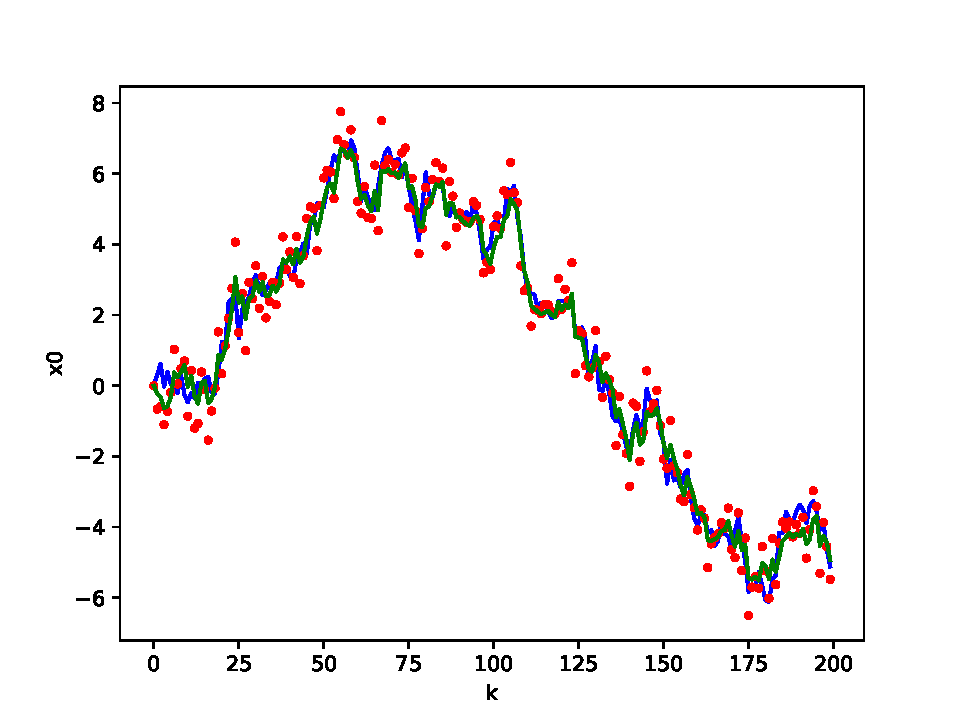
\includegraphics[width=0.75\textwidth,height=\textheight]{AdvFilteringFigures/kalmandemo2_x.*}
\caption{}
\end{figure}

The blue dots are a graph of \((x_2)_k\), and the green dots are the
Kalman estimate of the state.

\begin{figure}
\centering
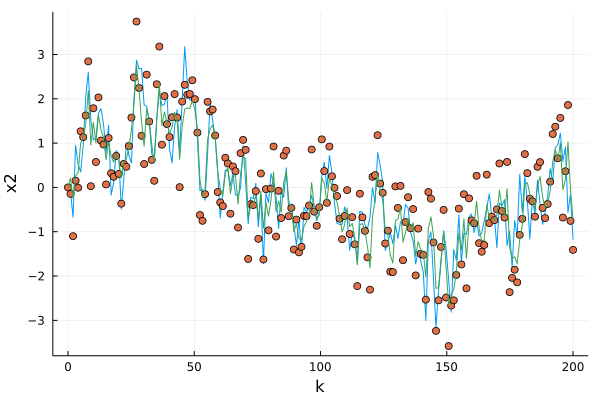
\includegraphics[width=0.75\textwidth,height=\textheight]{AdvFilteringFigures/kalmandemo2_y.*}
\caption{}
\end{figure}

What happens if we can only observe one state? What if

\[H = \begin{bmatrix} 1& 0  \end{bmatrix}\]

In this example, we will also make the simplications in the code that
you would do in practice. For example, when you see \(Hx\) you would
just code up \(x_1\).

\begin{Shaded}
\begin{Highlighting}[]
\KeywordTok{using} \BuiltInTok{Random}\OperatorTok{,}\NormalTok{ Distributions}
\KeywordTok{using}\NormalTok{ Plots}\OperatorTok{,}\NormalTok{ LinearAlgebra}
\end{Highlighting}
\end{Shaded}

The simulation variables ...

\begin{Shaded}
\begin{Highlighting}[]
\CommentTok{\#  Create fake dataset for experiment}
\NormalTok{N }\OperatorTok{=} \FloatTok{200}
\NormalTok{t }\OperatorTok{=}\NormalTok{ range(}\FloatTok{0}\OperatorTok{,} \FloatTok{10}\OperatorTok{,}\NormalTok{ length }\OperatorTok{=}\NormalTok{ N)  }\CommentTok{\# for control input}
\NormalTok{u1 }\OperatorTok{=} \FloatTok{0.75}\OperatorTok{*}\NormalTok{sin.(}\FloatTok{0.5}\OperatorTok{*}\NormalTok{t)}
\NormalTok{u2 }\OperatorTok{=} \FloatTok{0.5}\OperatorTok{*}\NormalTok{cos.(}\FloatTok{0.5}\OperatorTok{*}\NormalTok{t)}
\NormalTok{mu1 }\OperatorTok{=}\NormalTok{ [}\FloatTok{0.0}\OperatorTok{,} \FloatTok{0.0}\NormalTok{]}
\NormalTok{mu2 }\OperatorTok{=} \FloatTok{0.0}
\NormalTok{x\_sim }\OperatorTok{=}\NormalTok{ zeros(}\FloatTok{2}\OperatorTok{,}\NormalTok{ N)}
\NormalTok{z\_sim }\OperatorTok{=}\NormalTok{ zeros(N)}
\NormalTok{F }\OperatorTok{=} \DataTypeTok{Float64}\NormalTok{[}\FloatTok{0.85} \OperatorTok{{-}}\FloatTok{0.01}\OperatorTok{;} \FloatTok{0.02} \FloatTok{0.65}\NormalTok{]}
\NormalTok{FT }\OperatorTok{=}\NormalTok{ transpose(F)}
\NormalTok{G }\OperatorTok{=}\NormalTok{ transpose(}\DataTypeTok{Float64}\NormalTok{[u1 u2}\OperatorTok{;}\NormalTok{])}
\end{Highlighting}
\end{Shaded}

The filter variables

\begin{Shaded}
\begin{Highlighting}[]
\NormalTok{V }\OperatorTok{=} \DataTypeTok{Float64}\NormalTok{[}\FloatTok{0.2} \FloatTok{0.02}\OperatorTok{;} \FloatTok{0.02} \FloatTok{0.35}\NormalTok{]}
\NormalTok{W }\OperatorTok{=} \FloatTok{0.4}
\NormalTok{P }\OperatorTok{=}\NormalTok{ zeros(}\FloatTok{2}\OperatorTok{,}\FloatTok{2}\NormalTok{)}
\NormalTok{x\_estimate }\OperatorTok{=}\NormalTok{ zeros(}\FloatTok{2}\OperatorTok{,}\NormalTok{N)}
\end{Highlighting}
\end{Shaded}

The simulation ...

\begin{Shaded}
\begin{Highlighting}[]
\KeywordTok{for}\NormalTok{ k }\OperatorTok{=} \FloatTok{2}\OperatorTok{:}\NormalTok{N}
\NormalTok{  process\_noise }\OperatorTok{=}\NormalTok{ rand(MvNormal(mu1}\OperatorTok{,}\NormalTok{ V)}\OperatorTok{,} \FloatTok{1}\NormalTok{)}
\NormalTok{  observation\_noise }\OperatorTok{=}\NormalTok{ rand(Normal(mu2}\OperatorTok{,}\NormalTok{ W[}\FloatTok{1}\NormalTok{]))}
\NormalTok{  x\_sim[}\OperatorTok{:,}\NormalTok{k] }\OperatorTok{=}\NormalTok{ (F }\OperatorTok{*}\NormalTok{ x\_sim[}\OperatorTok{:,}\NormalTok{ k}\OperatorTok{{-}}\FloatTok{1}\NormalTok{]) }\OperatorTok{+}\NormalTok{ G[}\OperatorTok{:,}\NormalTok{k] }\OperatorTok{+}\NormalTok{ process\_noise}
\NormalTok{  z\_sim[k] }\OperatorTok{=}\NormalTok{ x\_sim[}\FloatTok{1}\OperatorTok{,}\NormalTok{ k] }\OperatorTok{+}\NormalTok{ observation\_noise}
 \KeywordTok{end}
 \CommentTok{\# done with fake data}
\end{Highlighting}
\end{Shaded}

The code block above provides the array z which is then piped into the
Kalman Filter

\begin{Shaded}
\begin{Highlighting}[]
\KeywordTok{for}\NormalTok{ k }\OperatorTok{=} \FloatTok{2}\OperatorTok{:}\NormalTok{N}
\NormalTok{  x\_process\_update }\OperatorTok{=}\NormalTok{ F }\OperatorTok{*}\NormalTok{ x\_estimate[}\OperatorTok{:,}\NormalTok{k}\OperatorTok{{-}}\FloatTok{1}\NormalTok{] }\OperatorTok{+}\NormalTok{ G[}\OperatorTok{:,}\NormalTok{k]}
\NormalTok{  P\_variance\_update }\OperatorTok{=}\NormalTok{ F }\OperatorTok{*}\NormalTok{ (P }\OperatorTok{*}\NormalTok{ FT) }\OperatorTok{+}\NormalTok{ V}
\NormalTok{  innovation }\OperatorTok{=}\NormalTok{ z\_sim[k] }\OperatorTok{{-}}\NormalTok{ x\_process\_update[}\FloatTok{1}\NormalTok{]}
\NormalTok{  Innovation\_covariance }\OperatorTok{=}\NormalTok{ P\_variance\_update[}\FloatTok{1}\OperatorTok{,}\FloatTok{1}\NormalTok{] }\OperatorTok{+}\NormalTok{ W}
\NormalTok{  Kal\_gain }\OperatorTok{=}\NormalTok{ (}\FloatTok{1.0}\OperatorTok{/}\NormalTok{Innovation\_covariance) }\OperatorTok{.*}\NormalTok{ P\_variance\_update[}\OperatorTok{:,}\FloatTok{1}\NormalTok{]}
\NormalTok{  x\_estimate[}\OperatorTok{:,}\NormalTok{k] }\OperatorTok{=}\NormalTok{ x\_process\_update }\OperatorTok{+}\NormalTok{ innovation }\OperatorTok{.*}\NormalTok{ Kal\_gain}
\NormalTok{  P }\OperatorTok{=}\NormalTok{ P\_variance\_update }\OperatorTok{{-}}\NormalTok{ Kal\_gain }\OperatorTok{*}\NormalTok{ transpose(P\_variance\_update[}\FloatTok{1}\OperatorTok{,:}\NormalTok{] )}
\KeywordTok{end}
\end{Highlighting}
\end{Shaded}

\begin{Shaded}
\begin{Highlighting}[]
\NormalTok{time }\OperatorTok{=}\NormalTok{ range(}\FloatTok{0}\OperatorTok{,}\NormalTok{ N}\OperatorTok{,}\NormalTok{ length}\OperatorTok{=}\NormalTok{N)}
\NormalTok{p1 }\OperatorTok{=}\NormalTok{ plot(time}\OperatorTok{,}\NormalTok{ x\_sim[}\FloatTok{1}\OperatorTok{,:}\NormalTok{]}\OperatorTok{,}\NormalTok{ xlabel }\OperatorTok{=} \StringTok{"k"}\OperatorTok{,}\NormalTok{ ylabel }\OperatorTok{=} \StringTok{"x1"}\OperatorTok{,}\NormalTok{ legend }\OperatorTok{=} \ExtensionTok{false}\NormalTok{)}
\NormalTok{scatter}\OperatorTok{!}\NormalTok{(time}\OperatorTok{,}\NormalTok{z\_sim)}
\NormalTok{plot}\OperatorTok{!}\NormalTok{(time}\OperatorTok{,}\NormalTok{x\_estimate[}\FloatTok{1}\OperatorTok{,:}\NormalTok{])}
\NormalTok{display(p1)}
\NormalTok{savefig(}\StringTok{"kalmandemo3\_x.svg"}\NormalTok{)}

\NormalTok{p2 }\OperatorTok{=}\NormalTok{ plot(time}\OperatorTok{,}\NormalTok{ x\_sim[}\FloatTok{2}\OperatorTok{,:}\NormalTok{]}\OperatorTok{,}\NormalTok{ xlabel }\OperatorTok{=} \StringTok{"k"}\OperatorTok{,}\NormalTok{ ylabel }\OperatorTok{=} \StringTok{"x2"}\OperatorTok{,}\NormalTok{ legend }\OperatorTok{=} \ExtensionTok{false}\NormalTok{)}
\NormalTok{plot}\OperatorTok{!}\NormalTok{(time}\OperatorTok{,}\NormalTok{x\_estimate[}\FloatTok{2}\OperatorTok{,:}\NormalTok{])}
\NormalTok{display(p2)}
\NormalTok{savefig(}\StringTok{"kalmandemo3\_y.svg"}\NormalTok{)}
\end{Highlighting}
\end{Shaded}

The blue line is the graph of \((x_1)_k\), the red dots are the
observations \(z_k\), and the green line is the Kalman estimate of the
state.

\begin{figure}
\centering
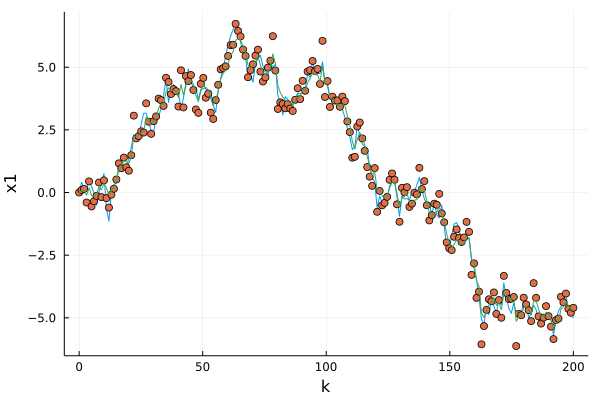
\includegraphics[width=0.75\textwidth,height=\textheight]{AdvFilteringFigures/kalmandemo3_x.*}
\caption{}
\end{figure}

The blue line is the graph of \((x_2)_k\), and the red line are the
Kalman estimate of the state.

\begin{figure}
\centering
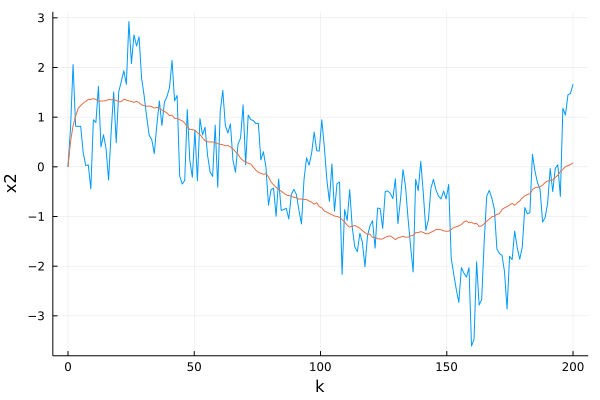
\includegraphics[width=0.75\textwidth,height=\textheight]{AdvFilteringFigures/kalmandemo3_y.*}
\caption{}
\end{figure}

\hypertarget{injecting-noise}{%
\subsection{Injecting noise}\label{injecting-noise}}

You may have noticed that we have added noise to the end of the
expression. Why add? Why not multiply? Assume that we have two signals

\[a(t) = \cos(t) , \quad  b(t) = 20\cos(t)\]

and to them we add mean zero Gaussian noise with standard deviation
\(\sigma = 0.25\), \(v\):

\[a_1(t) = \cos(t) +v, \quad  b_1(t) = 20\cos(t) + v\]

or we multiply that noise

\[a_2(t) = v\cos(t), \quad  b_2(t) = 20v\cos(t)\]

We then subtract off the signal and compute the standard deviations. For
\(a_1\) and \(b_1\), it is mathematically clear that you would get
\(\sigma = 0.25\) back - if the sample size large enough.

\begin{Shaded}
\begin{Highlighting}[]
\NormalTok{t }\OperatorTok{=}\NormalTok{ range(}\FloatTok{0}\OperatorTok{,}\FloatTok{6.28}\OperatorTok{,}\NormalTok{length}\OperatorTok{=}\NormalTok{N)}
\NormalTok{c }\OperatorTok{=}\NormalTok{ cos.(t)}
\NormalTok{n }\OperatorTok{=}\NormalTok{ rand(Normal(}\FloatTok{0}\OperatorTok{,} \FloatTok{0.25}\NormalTok{)}\OperatorTok{,} \FloatTok{200}\NormalTok{)}
\NormalTok{a1 }\OperatorTok{=}\NormalTok{ c }\OperatorTok{+}\NormalTok{ n}
\NormalTok{b1 }\OperatorTok{=} \FloatTok{20} \OperatorTok{*}\NormalTok{ c }\OperatorTok{+}\NormalTok{ n}
\NormalTok{a2 }\OperatorTok{=}\NormalTok{ n }\OperatorTok{.*}\NormalTok{ c}
\NormalTok{b2 }\OperatorTok{=} \FloatTok{20} \OperatorTok{*}\NormalTok{ n }\OperatorTok{.*}\NormalTok{ c}
\NormalTok{a1sub }\OperatorTok{=}\NormalTok{ a1 }\OperatorTok{{-}}\NormalTok{ c}
\NormalTok{b1sub }\OperatorTok{=}\NormalTok{ b1 }\OperatorTok{{-}} \FloatTok{20} \OperatorTok{*}\NormalTok{ c}
\NormalTok{a2sub }\OperatorTok{=}\NormalTok{ a2 }\OperatorTok{{-}}\NormalTok{ c}
\NormalTok{b2sub }\OperatorTok{=}\NormalTok{ b2 }\OperatorTok{{-}} \FloatTok{20} \OperatorTok{*}\NormalTok{ c}
\NormalTok{std(a1sub)}
\NormalTok{std(b1sub)}
\NormalTok{std(a2sub)}
\NormalTok{std(b2sub)}
\end{Highlighting}
\end{Shaded}

The output

\begin{Shaded}
\begin{Highlighting}[]
\NormalTok{julia}\OperatorTok{\textgreater{}}\NormalTok{ std(a1sub)}
\FloatTok{0.24006607075812747}

\NormalTok{julia}\OperatorTok{\textgreater{}}\NormalTok{ std(b1sub)}
\FloatTok{0.24006607075812744}

\NormalTok{julia}\OperatorTok{\textgreater{}}\NormalTok{ std(a2sub)}
\FloatTok{0.7324916532871306}

\NormalTok{julia}\OperatorTok{\textgreater{}}\NormalTok{ std(b2sub)}
\FloatTok{14.649833065742614}
\end{Highlighting}
\end{Shaded}

The multiplication by the signal will amplify the noise by the signal
strength and this changes the effective standard deviation. We will for
this text focus on adding noise via addition. At this point, if you look
at what we just did, it is actually pretty obvious. In the additive case
we have

\[(x + v) - x = v\]

One issue we will address later in this chapter is the difference
between process noise and control noise. By process noise we mean the
addition of noise in the process step, the addition of \(v\):

\[x_{k+1} = Fx_k + Gu_k + v_k .\]

Noise in the control would appear as \(u_k + r_k\) where \(r_k\) is some
zero mean noise term. This would get changed by the term \(G\)

\[x_{k+1} = Fx_k + G(u_k + r_k)  + v_k  = Fx_k + Gu_k + Gr_k  + v_k  = Fx_k + Gu_k + v'_k .\]

For now, we just assume we can lump the two together with a modified
process noise term.

\hypertarget{the-classic-vehicle-on-track-example}{%
\subsection{The Classic Vehicle on Track
Example}\label{the-classic-vehicle-on-track-example}}

Consider a mobile robot along a track. Let the state \(x = [x_r , s_r]\)

where \(x_r\) and \(s_r\) are the vehicle position and speed. Let \(m\)

denote the mass of the vehicle and \(u\) be the force acting on the
vehicle. Note that

\[\frac{ds_r}{dt} = \frac{u}{m}\]

Discretize

\[\frac{s_r(t+T)-s_r(t)}{T} \approx \frac{ds_r}{dt}\]

\(T\) is the sample rate. Thus

\[s_r(k+1) = s_r(k) + \frac{T}{m} \, u(k).\]

From calculus we know that

\[\frac{dx_r}{dt} = s_r.\]

Discretizing this equation

\[\frac{dx_r}{dt} \approx \frac{x_r(k+1) - x_r(k)}{T} =  s_r(k)\]

and rewriting gives

\[x_r(k+1) = x_r(k) + T s_r(k).\]

This gives the pair of equations

\[\begin{aligned}
\begin{array}{l}
x_r(k+1) = x_r(k) + T s_r(k) \\
s_r(k+1) = s_r(k) + \frac{T}{m} \, u(k)
\end{array}
\end{aligned}\]

Load the variables into an array

\[\begin{aligned}
x_{k+1} = \begin{bmatrix}1 & T \\ 0 & 1\end{bmatrix} x_k
  + \begin{bmatrix} 0 \\ T/m \end{bmatrix}u_k + v_k
\end{aligned}\]

Assume that you have some sensors

\[z_{k+1} = \begin{bmatrix}0 & 1\end{bmatrix} x_k + w_k\]

where \(v\) and \(w\) are zero mean Gaussian noise. Thus

\[\begin{aligned}
F_k = \begin{bmatrix} 1 & T \\ 0 & 1\end{bmatrix}, \quad
  G_k = \begin{bmatrix} 0 \\ T/m \end{bmatrix}, \quad
  H_k = \begin{bmatrix} 0 & 1\end{bmatrix}
\end{aligned}\]

For this example take \(m=1\) and \(T=0.5\). Assume the covariance of
\(v_k\)

\[\begin{aligned}
V_k = \begin{bmatrix}0.2 & 0.05 \\ 0.05 & 0.1\end{bmatrix}
\end{aligned}\]

Assume the covariance for \(w_k\) is \(W_k = [0.5]\), and at \(k=0\),
\(u(0) = 0\) and
\(\hat{x}_{0|0} = \begin{bmatrix}2 & 4\end{bmatrix}^T\),

\[\begin{aligned}
P_{0|0}
        = \begin{bmatrix}1 & 0 \\ 0 & 2\end{bmatrix}
\end{aligned}\]

Next we compute one iteration of the Kalman Filter.

\begin{itemize}
\item
  State estimate prediction:

  \[\begin{aligned}
  \hat{x}_{1|0} = F_{1}\hat{x}_{0|0} + G_{1} u_{1} =
  \begin{bmatrix}1 & 0.5 \\ 0 & 1\end{bmatrix}
              \begin{bmatrix}2 \\4 \end{bmatrix} + \begin{bmatrix}0
                \\ 0.5\end{bmatrix} 0 =
  \begin{bmatrix}4 \\ 4\end{bmatrix}
  \end{aligned}\]
\item
  Covariance prediction

  \[P_{1|0} = F_{1} P_{0|0} F_{1}^{T} + V_{1}\]

  \[\begin{aligned}
  = \begin{bmatrix}1 & 0.5 \\ 0 & 1\end{bmatrix}
  \begin{bmatrix}1 & 0 \\ 0 & 2\end{bmatrix}
  \begin{bmatrix}1 & 0 \\ 0.5 & 1\end{bmatrix} +
  \begin{bmatrix}0.2 & 0.05 \\ 0.05 & 0.1\end{bmatrix}
  = \begin{bmatrix}1.7 & 1.05 \\ 1.05 & 2.1\end{bmatrix}
  \end{aligned}\]
\end{itemize}

Assume that you measure and obtain

\[z_1 = 3.8\]

\begin{itemize}
\item
  Innovation:

  \[\begin{aligned}
  y_k = z_1 - H\hat{x}_{1|0} = 3.8 - \begin{bmatrix} 0 & 1\end{bmatrix}
  \begin{bmatrix}4 \\ 4\end{bmatrix} = -.2
  \end{aligned}\]
\item
  The matrix \(S\)

  \[\begin{aligned}
  S_1 = H P_{1|0} H^\text{T} + W_1
  = \begin{bmatrix} 0 & 1\end{bmatrix} \begin{bmatrix}1.7 & 1.05 \\ 1.05 & 2.1\end{bmatrix}
  \begin{bmatrix}0 \\ 1\end{bmatrix} +0.5 = 2.6
  \end{aligned}\]
\item
  The matrix \(K\) (Kalman Gain)

  \[\begin{aligned}
  K_1 = P_{1|0}H^\text{T}S_1^{-1} = \begin{bmatrix}1.7 & 1.05 \\ 1.05 & 2.1\end{bmatrix}
  \begin{bmatrix}0 \\ 1\end{bmatrix}
  \left( 2.6 \right)^{-1} =
  \begin{bmatrix}0.404 \\ 0.808\end{bmatrix}
  \end{aligned}\]
\item
  The estimate update:

  \[\begin{aligned}
  \hat{x}_{1|1} = \hat{x}_{1|0} + K_1 y_1 =\begin{bmatrix}4 \\ 4\end{bmatrix} +\begin{bmatrix}0.404 \\ 0.808\end{bmatrix}(-.2) = \begin{bmatrix}3.9192 \\ 3.8384 \end{bmatrix}
  \end{aligned}\]
\item
  The covariance estimate update:

  \[P_{1|1} = (I - K_1 H) P_{1|0}\]

  \[\begin{aligned}
  = \left( \begin{bmatrix}1 & 0 \\ 0& 1\end{bmatrix}
  -  \begin{bmatrix}0.404 \\ 0.808\end{bmatrix} \begin{bmatrix} 0 & 1\end{bmatrix} \right)
  \begin{bmatrix}1.7 & 1.05 \\ 1.05 & 2.1\end{bmatrix}
  =\begin{bmatrix}.4242 & .8484 \\ .8484 & 1.6968\end{bmatrix}
  \end{aligned}\]
\end{itemize}

\hypertarget{the-kalman-gain}{%
\subsection{The Kalman Gain}\label{the-kalman-gain}}

The Kalman Gain selects the amount of process update to be used compared
to the amount of observation to be used. It is weighting each one to
produce the best possible estimate of state based on the current
understanding of the errors on both.

The Kalman Gain can be written as

\[K_k = P_{k}H_k^\text{T}\left( H_k P_{k} H_k^\text{T} + W_k \right)^{-1}.\]

If all of these variables were \emph{scalars}, we can get a feel for the
bounds on the Kalman Gain:

\[K_k = P_{k}H_k / \left( H_k^2 P_{k} + W_k \right)\]

When \(W_k = 0\) then \(K_k = 1/H_k\) and as \(W_k \to \infty\) then
\(K_k = 0\), so \(0 < K_k < 1/H_k\).

\hypertarget{some-issues-to-address}{%
\subsection{Some issues to address}\label{some-issues-to-address}}

Because the Kalman filter is trying to estimate the state, and determine
the process as well as the observation quality, the initial iterations
may be very inaccurate. Assuming you have a convergent process, it can
still take some time for the filter to converge and provide a good state
estimate. What the filter is doing is figuring out the errors for the
state estimate (the covariance \(P\)). Many robotics applications will
have the robot sit still for a few seconds to allow the filter to
converge.

A common question is what should the initial values be? For the state
estimate, one clearly uses starting information that one has. The
problem is that maybe not all the data is known. For unknown variables,
setting to zero is about all you can do. The corresponding entry in the
covariance matrix should be infinity (or a very large value). Another
approach for the covariance is to set it to zero and let the first dozen
iterations figure out the covariance or one can populate it with values.
One could even store the covariance after the filter settles and use
that to initialize the filter.

For matrix \(W\), we use the sensor datasheets which can provide
standard deviations for sensor readings. The squares of those can be
placed on the diagonal of \(W\). The matrix \(V\) is harder to determine
and may require some experimentation. A simplistic approach would be to
run the robot for a single step and measure the end state. Repeat this
process for a large enough times as possible. That endstate measurement
data can be used to determine the variances of the process as well as
can be used to adjust the process in case of parameter issues.

A variation on this approach for \(V\) is to run the robot in for
multiple time steps and do the statistics on the end state as before.
Another method is to compare the Kalman estimation with the actual state
(done by hand measurement and not onboard sensing). The tune the
parameters. You can then optimize to gain good choices for \(V\), \(W\).
It should be noted that \(V\) is the estimate for a given \(\Delta t\).
It needs to be scaled for time steps other than the one it was developed
for. So, if \(V\) was developed for a time step of \(\Delta t\) and the
Kalman estimation loops are using a time step of \(T\) , then
\(V' = (T/ \Delta t) V\) would scale the covariance.

One concern follows from unreliable sensor connections. What happens
when a sensor is down or is not sending data? The Kalman gain is the
term that selects the relative amount of the model verses the sensor to
use in the estimate. Lacking a sensor, the Kalman gain will after some
iterations shut off that sensor. It will do this even if the sensor is
operational if the sensor is giving readings that don't make sense given
the physical model, so the Kalman gain will move to where only the
physical model is used.

\[K_k = P_kH_k^TS_k^{-1} \to 0\]

This can be a problem for sensors that have drift or some type of
uncorrected deterministic error (DC bias).

The Kalman filter does not correct for drift that occurs in gyros and
other instruments. The common fix is to periodically reset (zero) the
sensor when in a known configuration - for example when the vehicle is
stopped and you know it is not turning. The issue of course is that
after a period of time the Kalman estimate becomes just the process
update step. The Kalman Gain parameter can be monitored. When it falls
below some threshold, then the sensor needs to be reset.

\hypertarget{work-estimates}{%
\subsubsection{Work Estimates}\label{work-estimates}}

If you have \(n\) equations, the work (multiplications) in the filter
is:

\begin{enumerate}
\tightlist
\item
  \(\hat{x}_{k|k-1} = F_{k}\hat{x}_{k-1|k-1} + G_{k} u_{k}\) : ~
  \(O(n^2)\)
\item
  \(P_{k|k-1} = F_{k} P_{k-1|k-1} F_{k}^{T} + V_{k}\) : ~\(O(n^3)\)
\item
  \(K_k = P_{k|k-1}H_k^\text{T}\left[ H_k P_{k|k-1} H_k^\text{T} + W_k  \right]^{-1}\)
  : ~\(O(m!)\) + \(O(n^2m)\)
\item
  \(\hat{x}_{k|k} =   \hat{x}_{k|k-1} + K_k \left(z_k - H_k\hat{x}_{k|k-1} \right)\)
  : ~\(O(n^2)\)
\item
  \(P_{k|k} =   (I - K_k H_k) P_{k|k-1}\) : ~\(O(n^3)\)
\end{enumerate}

The largest work is in step 3. By using an \(LU\) factorization, we can
move this down to \(\text{max}(O(m^3),O(n^2m))\) work. Step 2 can
exploit symmetry to reduce work as only 1/2 the matrix needs to be
computed. For small matrices, explicit formulas for the inverse can be
used.

\hypertarget{different-sensor-types}{%
\subsection{Different Sensor Types}\label{different-sensor-types}}

Now that we have the basic Kalman Filter process, we can look at some
variations on how it is applied. One question that arises is ``What
should we do if we have multiple sensors?'' Currently, the update stage
runs a single measurement fusion. The solution is to run the update loop
for each sensor. This is equivalent to running the full Kalman loop but
skipping the prediction step between the different sensors. The
algorithm follows.

\textbf{Predict:}

\begin{itemize}
\tightlist
\item
  \(\hat{x}_{k|k-1} = F_{k}\hat{x}_{k-1|k-1} + G_{k} u_{k}\)
\item
  \(P_{k|k-1} = F_{k} P_{k-1|k-1} F_{k}^{T} + V_{k}\)
\end{itemize}

\textbf{Update:}

\begin{itemize}
\tightlist
\item
  foreach sensor \(i\):

  \begin{itemize}
  \tightlist
  \item
    \(y_k = z_k^i - (H^i)_k\hat{x}_{k|k-1}\)
  \item
    \(S_k = (H^i)_k P_{k|k-1} (H^i)_k^\text{T} + W_k^i\)
  \item
    \(K_k = P_{k|k-1}(H^i)_k^\text{T}S_k^{-1}\)
  \item
    \(\hat{x}_{k|k-1} = \hat{x}_{k|k-1} + K_k y_k\)
  \item
    \(P_{k|k-1} = (I - K_k (H^i)_k) P_{k|k-1}\)
  \end{itemize}
\item
  \(\hat{x}_{k|k} = \hat{x}_{k|k-1}\)
\item
  \(P_{k|k} = P_{k|k-1}\)
\end{itemize}

From this algorithm we notice that we have the ability to fuse multiple
different sensors; meaning you have multiple sensors measuring a single
state \(x_k\). Using the update steps we can fuse sensor measurements
without the need to perform the prediction step. Sensor fusion can be
done using a simplification of the Kalman Filter. Since we only have
observations, \(F=I\), \(G=0\), \(V=0\) and so the apriori stage of the
filter drops out: So, we can just skip the apriori step. This means we
can define \(\hat{x}_{k}  = \hat{x}_{k|k}\) and \(P_{k} = P_{k|k}\) and
we have a basic formula to merge the sensed data. Since we don't have
the time loop (in \(k\)), we can redefine \(k\) to loop over the
sensors. This reduces to exactly the sensor fusion algorithm given in
\texttt{multivariatesensorfusion}.

In the last section we discussed the issue regarding unreliable sensor
readings in the situation where the data is occasionally not available.
This brings up a concern about having the data ready when the update
step is done. The assumption so far was that the Kalman loop is run at
the same frequency that the data is arriving.

However, there are several situations for which this is a problem. One
such situation is when several different classes of sensors are being
used. For example, your magnetometer may run at 80 Hz and your Lidar
might operate at 10 Hz. One solution is to run at 10Hz and just skip the
extra measurements from the magnetometer. Another possible problem
arises when the time between the sensor readings are very long giving a
\(\Delta t\) that is very large. A large \(\Delta t\) can make the
predictive step inaccurate.

\textbf{Predict:}

\begin{itemize}
\tightlist
\item
  \(\hat{x}_{k|k-1} = F_{k}\hat{x}_{k-1|k-1} + G_{k} u_{k}\)
\item
  \(P_{k|k-1} = F_{k} P_{k-1|k-1} F_{k}^{T} + V_{k}\)
\end{itemize}

\textbf{Update:}

\begin{itemize}
\tightlist
\item
  Loop over available sensor data during \(\Delta t\) :

  \begin{itemize}
  \tightlist
  \item
    \(y_k = z_k^i - (H^i)_k\hat{x}_{k|k-1}\)
  \item
    \(S_k = (H^i)_k P_{k|k-1} (H^i)_k^\text{T} + W_k^i\)
  \item
    \(K_k = P_{k|k-1}(H^i)_k^\text{T}S_k^{-1}\)
  \item
    \(\hat{x}_{k|k-1} = \hat{x}_{k|k-1} + K_k y_k\)
  \item
    \(P_{k|k-1} = (I - K_k (H^i)_k) P_{k|k-1}\)
  \end{itemize}
\item
  \(\hat{x}_{k|k} = \hat{x}_{k|k-1}\)
\item
  \(P_{k|k} = P_{k|k-1}\)
\end{itemize}

\textbf{Footnotes}
